% ------------------------------------------------------------------------------
% TYPO3 Version 10.0 - What's New (English Version)
%
% @author	Michael Schams <schams.net>
% @license	Creative Commons BY-NC-SA 3.0
% @link		http://typo3.org/download/release-notes/whats-new/
% @language	English
% ------------------------------------------------------------------------------

\section{Modifiche per integratori}
\begin{frame}[fragile]
	\frametitle{Modifiche per integratori}

	\begin{center}\huge{Capitolo 3:}\end{center}
	\begin{center}\huge{\color{typo3darkgrey}\textbf{Modifiche per integratori}}\end{center}

\end{frame}

% ------------------------------------------------------------------------------
% TYPO3 Version 10.0 - Breaking Changes

\begin{frame}[fragile]
	\frametitle{Changes for Integrators}
	\framesubtitle{Modifiche importanti}

	\small
		Informazione per gli integratori: in TYPO3 v9, parti di codice PHP, TSconfig, TypoScript
		opzioni e condizioni, nonché la pianificazione dello scheduler sono stati segnati come deprecati.

		\vspace{0.2cm}

		In conformità alla \textbf{deprecation policy} di TYPO3, questi componenti sono stati
		modificati o rimossi in TYPO3 v10.0.

		\vspace{0.2cm}

		Abilitate il deprecation log, verificate attentamente il vostro codice ed esaminate i log per
		individuare possibili problemi. Usate l'
		\href{https://docs.typo3.org/m/typo3/reference-coreapi/master/en-us/ApiOverview/ExtensionScanner/Index.html}{Extension Scanner}
		integrato per ottenere un rapporto completo delle incompatibilità delle estensioni.

	\normalsize

\end{frame}

% ------------------------------------------------------------------------------
% Feature | 78432 | Add log message for Switch User action

\begin{frame}[fragile]
	\frametitle{Changes for Integrators}
	\framesubtitle{Cambio utente di Backend}

	\begin{itemize}
		\item Un messagio viene scritto nei log se un amministratore cambia in un altro utente di backend:
	\end{itemize}

	\begin{figure}
		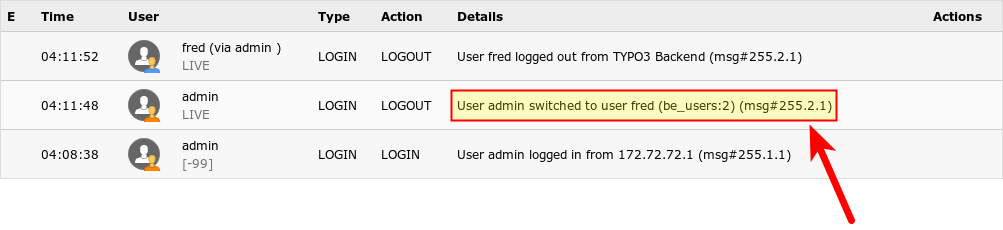
\includegraphics[width=0.90\linewidth]{ChangesForIntegrators/78432-SwitchUserActionLogMessage.png}
	\end{figure}

\end{frame}

% ------------------------------------------------------------------------------
% Feature | 83734 | Add support for current page in configcache
% Breaking | 88564 | PageTSconfig setting TSFE.constants removed
% Breaking | 88657 | Popup configuration in FormEngine dropped

\begin{frame}[fragile]
	\frametitle{Changes for Integrators}
	\framesubtitle{Cambiameti TypoScript}

	\begin{itemize}
		\item La proprietà TypoScript \texttt{config.cache} supporta ora la parola chiave
			"\texttt{current}" per fare riferimento alla pagina corrente. Per esempio:\newline
			\smaller\texttt{config.cache.all = fe\_users:current}\normalsize

		\item L'impostazione Page/User TSconfig \texttt{TSFE.constants} è stata rimossa.

			\begin{itemize}\smaller
				\item[\ding{228}] Includi le condizioni TypoScript in setup/constants e usa una corretta configurazione in \texttt{ext\_localconf.php}.
			\end{itemize}

		\item Le seguenti due configurazioni per impostare le dimensioni delle finestre popup sono state rimosse:

			\begin{itemize}
				\item \texttt{options.popupWindowSize}
				\item \texttt{options.rte.popupWindowSize}
			\end{itemize}

	\end{itemize}

\end{frame}

% ------------------------------------------------------------------------------
% Breaking | 88640 | Database field sys_template.nextLevel and TypoScript sublevel inheritance removed
% Task | 88755 | Remove POST option from typolink.addQueryString

\begin{frame}[fragile]
	\frametitle{Changes for Integrators}
	\framesubtitle{Cambiamenti TypoScript}

	\begin{itemize}
		\item Il campo \texttt{nextLevel} della tabella di database
			\texttt{sys\_template} è stato rimosso.

			\begin{itemize}\smaller
				\item[\ding{228}] Sostituisci il record (l'UID memorizzato nel campo \texttt{nextLevel}) con una condizione TypoScript da aggiungere per le sottopagine. Per esempio: \texttt{[tree.level > 1]}
			\end{itemize}\normalsize

		\item I seguenti valori non sono \textbf{più permessi}:

			\begin{itemize}\smaller
				\item \texttt{typolink.addQueryString.method = POST}
				\item \texttt{typolink.addQueryString.method = GET,POST}
				\item \texttt{typolink.addQueryString.method = POST,GET}
			\end{itemize}\normalsize

			\begin{itemize}\smaller
				\item[\ding{228}] Cambia le assegnazioni in TypoScript, Fluid e PHP in \texttt{GET}.
			\end{itemize}\normalsize

	\end{itemize}

\end{frame}

% ------------------------------------------------------------------------------
% Breaking | 87583 | Remove obsolete APC Cache Backend implementation
% Breaking | 87558 | Consolidate extbase caches

\begin{frame}[fragile]
	\frametitle{Changes for Integrators}
	\framesubtitle{Caches}

	% decrease font size for code listing
	\lstset{basicstyle=\tiny\ttfamily}

	\begin{itemize}
		\item Il framework di Caching non supporta più \texttt{ApcBackend}

			\begin{itemize}\smaller
				\item[\ding{228}] Usa \textbf{APCu} al suo posto - nota la "u".
			\end{itemize}

\begin{lstlisting}
VECCHIO:
$GLOBALS['TYPO3_CONF_VARS']['SYS']['caching']['cacheConfigurations']['rootline']['backend'] =
\TYPO3\CMS\Core\Cache\Backend\ApcBackend::class;

NUOVO:
$GLOBALS['TYPO3_CONF_VARS']['SYS']['caching']['cacheConfigurations']['rootline']['backend'] =
\TYPO3\CMS\Core\Cache\Backend\ApcuBackend::class;
\end{lstlisting}

		\item Le cache di Extbase \texttt{extbase\_reflection} e \texttt{extbase\_datamapfactory\_datamap}
			sono state consolidate e sono ora disponibili come singola cache chiamata "\texttt{extbase}".

	\end{itemize}

\end{frame}

% ------------------------------------------------------------------------------
% Breaking | 87009 | Use multiple translation files by default in EXT:form

\begin{frame}[fragile]
	\frametitle{Changes for Integrators}
	\framesubtitle{Form Framework}

	% decrease font size for code listing
	\lstset{basicstyle=\tiny\ttfamily}

	\begin{itemize}
		\item La seguente opzione è stata rinominata:\newline
			\small\texttt{translationFile} \textrightarrow\hspace{0.1cm}\texttt{translationFiles}\normalsize
		\item I file di traduzione di default sono ora registrati all'indice 10:

			\begin{itemize}
				\item \texttt{EXT:form/Resources/Private/Language/locallang.xlf}
				\item \texttt{EXT:form/Resources/Private/Language/Database.xlf}
			\end{itemize}

		\item I file personalizzati di configurazione YAML del form devono essere aggiornati.

\begin{lstlisting}
VECCHIO:
translationFile: path/to/locallang.xlf

NUOVO:
translationFiles:
  20: path/to/locallang.xlf
\end{lstlisting}

	\end{itemize}

\end{frame}

% ------------------------------------------------------------------------------
% xxxxx | Cache Storage Type

\begin{frame}[fragile]
	\frametitle{Changes for Integrators}
	\framesubtitle{Tipo di archiviazione della Cache (1)}

	\begin{itemize}

		\item TYPO3 presenta un sistema di memorizzazione nella cache flessibile, con una
		    configurazione predefinita che è l'ideale per la maggior parte dei casi d'uso.
		\item Ora è possibile configurare il tipo di archiviazione per ottimizzare la cache
		    e aumentare le prestazioni in base al singolo ambiente.

			\begin{itemize}
				\item Scegli l'archivio \textbf{database} per un ambiente standard o se ad
					esempio viene utilizzato un file system di rete (NFS).
				\item Scegli \textbf{file system} se, ad esempio, viene utilizzata un'installazione
				    di database distribuita.
				\item Scegli \textbf{impostazioni della cache personalizzate} per configurare il tipo
				    di archiviazione per ogni cache in modo indipendente.
			\end{itemize}

		\item Per installazioni più complesse, dovrebbero essere considerate cache memory-based come
			\href{https://redis.io/}{Redis}
			o
			\href{https://memcached.org/}{Memcached}.

	\end{itemize}

\end{frame}

% ------------------------------------------------------------------------------
% xxxxx | Cache Storage Type

\begin{frame}[fragile]
	\frametitle{Changes for Integrators}
	\framesubtitle{Tipo di archiviazione della Cache (2)}

	\begin{itemize}

		\item Backend: \textbf{MAINTENANCE} \ding{223}\hspace{0.1cm}\textbf{Settings} \ding{223}\hspace{0.1cm}\textbf{Cache}:
		\end{itemize}

	\begin{figure}
		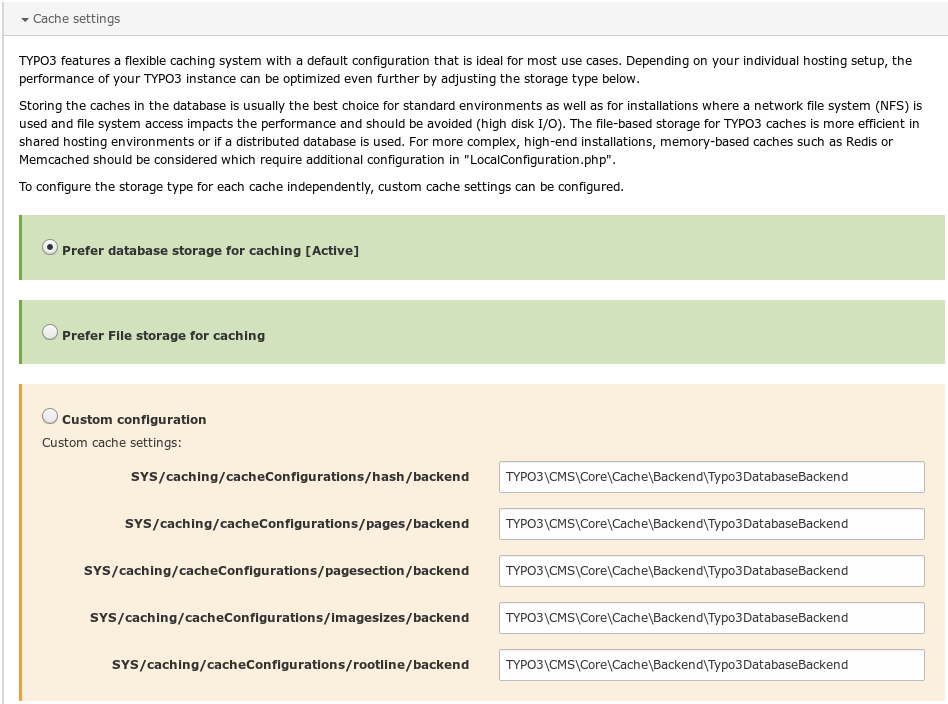
\includegraphics[width=0.60\linewidth]{ChangesForIntegrators/xxxxx-CacheStorageType.png}
	\end{figure}

\end{frame}

% ------------------------------------------------------------------------------
% 87499 | Drop extensions "taskcenter" and "sys_action" from core

\begin{frame}[fragile]
	\frametitle{Changes for Integrators}
	\framesubtitle{Task Center e \texttt{EXT:sys\_action}}

	\begin{itemize}

		\item Le estensioni di sistema \texttt{EXT:taskcenter} e \texttt{EXT:sys\_action}
			sono state rimosse dal core.

		\item Sono ora disponibili come estensioni separate nel
			\href{https://extensions.typo3.org/}{TER}
			e su
			\href{https://github.com/FriendsOfTYPO3}{GitHub}.

		\item Tieni d'occhio
			\href{https://typo3.org/community/teams/typo3-development/initiatives/typo3-dashboard-initiative/}{Iniziative Dashboard}
			per un approcio nuovo e migliore.

	\end{itemize}

\end{frame}

% ------------------------------------------------------------------------------
% Feature | 88648 | Define Twitter Card Type In Page Properties
% Important | 86577 | Query parameters are now included in canonicalized URLs

\begin{frame}[fragile]
	\frametitle{Changes for Integrators}
	\framesubtitle{Varie}

	% decrease font size for code listing
	\lstset{basicstyle=\tiny\ttfamily}

	\begin{itemize}

		\item Il tipo di Twitter Card può essere selezionato/configurato.
			Questa opzione imposta il meta tag \texttt{twitter:card} nel frontend.

\begin{lstlisting}
page {
  meta {
    twitter:card = summary_large_image
    twitter:card.replace = 1
  }
}
\end{lstlisting}

		\item Solo i parametri necessari per il cHash sono inclusi negli URL canonical, per impostazione predefinita.
			E' ora possibile configurare parametri di url aggiuntivi:

\begin{lstlisting}
$GLOBALS['TYPO3_CONF_VARS']['FE']['additionalCanonicalizedUrlParameters'].
\end{lstlisting}

		\smaller
			Nota: aggiungi solo parametri necessari a cambiare i contenuti della tua pagina. Altrimenti i motori di ricerca probabilmente classificheranno le tue pagine come contenuti duplicati.
		\normalsize

	\end{itemize}

\end{frame}

% ------------------------------------------------------------------------------
% Breaking | 88681 | Import Of PHP Files In Import Export Files Removed
% Breaking | 88500 | RTE image handling functionality dropped
% Breaking | 81950 | Remove leftover workspaces unpublishing functionality

\begin{frame}[fragile]
	\frametitle{Changes for Integrators}
	\framesubtitle{Varie}

	% decrease font size for code listing
	\lstset{basicstyle=\tiny\ttfamily}

	\begin{itemize}

		\item Quando si importano dati XML utilizzando \texttt{EXT:impexp}, il File Deny Pattern viene applicato
			e, ad esempio, rifiuta i file PHP incorporati.

		\item La funzionalità di gestione delle immagini in RTE è stata completamente rimossa.
			Per il supporto delle immagini in CKEditor, considera ad esempio l'uso di \texttt{EXT:rte\_ckeditor\_image}.

		\item La proprietà all'interno dei workspace per \textit{unpublishing} dei record è stata rimossa nella v10
			(incluso il campo del database \texttt{sys\_workspace.unpublish\_time}). Questa funzionalità era stata
			disabilitata in TYPO3 v4.5 e non più utilizzata o fornita dal core TYPO3.

	\end{itemize}

\end{frame}

% ------------------------------------------------------------------------------
% Breaking | 88772 | JavaScript script tags omit type=text/javascript in HTML5
% Remove system extension EXT:rsaauth
% Remove system extension EXT:fe_edit

\begin{frame}[fragile]
	\frametitle{Changes for Integrators}
	\framesubtitle{VArie}

	% decrease font size for code listing
	\lstset{basicstyle=\tiny\ttfamily}

	\begin{itemize}

		\item Quando l'output è in formato HTML5, i tag \texttt{<script>} non includono più
			l'attributo \texttt{type="text/javascript"}.

		\item Se necessario, questo può essere riattivato per il frontend usando TypoScript:

\begin{lstlisting}
page {
  includeJS {
    myfile = EXT:example/Resources/Public/JavaScript/myfile.js
    myfile.type = text/javascript
  }
}
\end{lstlisting}

		\item Le seguenti estensioni di sistema, deprecate, sono state rimosse:

			\begin{itemize}
				\item \texttt{EXT:rsaauth}
				\item \texttt{EXT:fe\_edit}
			\end{itemize}

	\end{itemize}

\end{frame}

% ------------------------------------------------------------------------------
